% !TeX root = ..\protokoll.tex
\documentclass[../protokoll.tex]{subfiles}
\graphicspath{{\subfix{../images/}}}
\begin{document}
\section{Nulleffekt}\label{sec:Nulleffekt}
In diesem Versuch wird der Nulleffekt $m_0$ des verwendeten Szintillationsdetektors gemessen. Dazu wird der Detektor wie in \ref{aufbau1} dargestellt aufgebaut.
\begin{figure}[h]
    \centering
    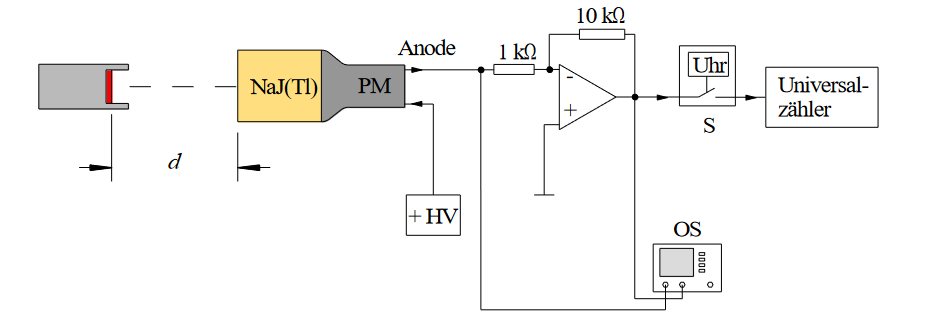
\includegraphics[width=0.7\textwidth]{2023-04-24 - V3 - Radioaktivität/images/versuch1/aufbau1.png}
    \caption{Schematischer Aufbau des Versuches, entnommen aus \cite{script}}
    \label{aufbau1}
\end{figure}
Der Photomultiplier des Detektors wird mit 1100 V von dem Hochspannungsgerät HV versorgt und die ausgehenden Signale werden mit einem Operationsverstärker verstärkt (die verwendeten Widerstände haben 10,06 $k\Omega$ und 1,012 $k\Omega$) und es werden beide Signale am Oszilloskop dargestellt. Der Aufbau ist mit einer Uhr und einem Universalzähler verbunden. Jedes Strahlungsereignis in dem an der Uhr eingestelltem Zeitraum wird an dem Zähler detektiert. Es wird die Hintergrundstrahlung gemessen, welche später aus der anderen Messung rausgerechnet wird. Dazu wird eine Messung für eine Zeit $\Delta t_0=120$ $s$ durchgeführt. Aus der mit dem Universalzähler gemessenen Impulszahl $M_0=8705$. Dadurch ergibt sich für $m_0=\frac{M_0}{\Delta t_0}=72,54$ $1/s$.
\end{document}